
\subsection{Magnetorquers  fault detection}
For magnetorquers fault detection, two types of structural analysis were implemented. First, a locally structure analysis for each magnetorquer was implemented, and second a second a structure analysis using the satellite dynamics.
\subsection{Magnetorquers local structural analysis} \label{sec: MTStructAnal}
Using the Biot-Savar law from \ref{eq:BS}, the residual for the magnetorquer is generated using the following equation:
\begin{flalign}
	residual = B - \frac{4 \mu_0}{\sqrt{2} \pi L} I
	\label{eq:BfS}
\end{flalign} 
where \\
$\vec B$ is the magnetic field \\
$\mu_0$ is a constant called permeability of free space \\
$I$ is the current \\
$L$ is the length of the coil

In equation \ref{eq:BfS} the magnetic field is measured and based on this measurement the magnetic moment can be deducted, but for the residual is not necessary, because if it is correct then the magnetic moment should be as expected using magnetic sensors for checking, unless the shape of the coil changes, perhaps due to some physical movement of the system.

\subsection{Unknown Input Observer (UIO)} \label{sec:UIO}
Uncertainties and modeling errors may cause discrepancies between the actual system and the descriptor mathematical model. Linearization and simplifications which make the system more manageable may lead also to uncertainties. All these\nomenclature[AU]{\textbf{UIO}}{Unknown Input Observer } uncertainties can have an effect on the system dynamic behavior through the input signals.   
A residual, fault indicator, based on observer design can be robust regarding the unknown input signals by making the effect of unknown inputs(UI) insensitive to the residual and thus making possible to maximize the detectability of a fault. The dynamic equation of the system can be written as 
%\nomenclature[A]{\textbf{UI}}{Unknown Input}
%

\begin{equation}
\dot{\vec{x}} = \underline A\vec{x}+\underline B \vec{u}+\underline E\vec{d}
\label{stateObs}
\end{equation}
\begin{equation}
\vec{y} = \underline C \vec{x}
\end{equation}
%
where $\underline A$ ,$\underline B$ and $ \underline C $ are the system matrix, input and output matrix respectively and $\underline E$ is the distribution matrix of the unknown input or disturbance vector $\vec{d}$. Furthermore, $\vec{x}$ is the state vector $\vec{u}$ is the input vector and $\vec{y}$ is the output vector. The time dependency of the variables has been suppressed in order to relax the notation. Following \cite{UIO}, 
%
%
\\
\textit{An observer is defined as Unknown Input Observer for a system described by \eqref{stateObs} if the state estimation error vector $e$ approaches zero asymptotically regardless of the presence of the unknown input }
\\
The full order observer
\begin{equation}
\dot{\vec{z}} = \underline F\vec{z}+\underline{TB} \vec{u}+\underline K\vec{y}
\label{stateObs1}
\end{equation}
\begin{equation}
\hat{\vec{x}} = \vec{z} + \underline H \vec{x}
\end{equation}
with $\hat{\vec{x}}$ be the state estimate and $\vec{z}$ the state of the observer. When \eqref{stateObs1} is an observer for the system given by \eqref{stateObs} the dynamics of the errors vector($\vec{e} = \vec{x} - \hat{\vec{x}}$) can be written as\cite{UIO} 
%
\begin{equation*}
\dot{\vec{e}}= (\underline A-\underline H \underline C \underline A-\underline K1 \underline C)\vec{e} + (\underline A-\underline H \underline C \underline A-\underline K1 \underline C - \underline F)\vec{z}+ ((\underline A-\underline H \underline C \underline A-\underline K1 \underline C )\underline H-\underline K2)\vec{y}
\label{errordynamics}
\end{equation*}
\begin{equation*}
+ (\underline I - \underline {HC} - \underline T)\underline B\vec{u}	+(\underline I -\underline H\underline C)\underline E \vec{d}
\label{errordynamics45}
\end{equation*}
in the above equation the utility of $\vec{x}  = \vec{e} + \hat{\vec{x}} = \vec{e} + \underline H\vec{y}+\vec{z}$ is used. The estimation error may converge to zero if the following conditions hold true:
%
\begin{equation}
\underline F = \underline A-\underline H \underline C \underline A-\underline K1 \underline C
\label{errordynamics3}
\end{equation}
\begin{equation}
(\underline I - \underline{HC})\underline E = 0
\label{errordynamics4}
\end{equation}
\begin{equation}
\underline T = (\underline I - \underline H\underline C)
\label{errordynamics5}
\end{equation}
\begin{equation}
\underline K = \underline K_{1} +\underline K_{2}
\label{errordynamics6}
\end{equation}
\begin{equation}
\underline K_{2} =\underline F \underline H 
\label{errordynamics7}
\end{equation}
where $\underline K_{1}$ is designed freely by pole placement to give desired eigenvalues of the observer. The error dynamics if the \ref{errordynamics4}...\ref{errordynamics7} hold true can now be written as 
\begin{equation}
\dot{\vec{e}} = \underline F \vec{e}
\label{errordynamics8}
\end{equation}
consequently if the eigenvalues of $\underline F$ are to the left half plane, the error converges exponentially asymptotically to zero. 

A solution to \eqref{errordynamics4} is given by making use of the Moore-Penrose pseudo-inverse as
\begin{equation}
\underline H = \underline E (\underline{CE})^\dagger
\label{errordynamics9}
\end{equation}
with $(\underline{CE})^{+} = [(\underline{CE})^{T} (\underline{CE})]^{-1}\underline{CE})^{T} $.
A sufficient and rather necessary conditions for the UIO existence is the number of independent unknown inputs can not be larger than the number of independent measurements which leads to
\begin{equation}
rank (\underline{CE}) =rank( \underline E) 
\label{errordynamics10}
\end{equation}
and by denoting $\underline A1 = \underline A - \underline{HCA} $ that the pair $(\underline {CA1})$ is detectable and thus $F$ can have stable roots.
\subsubsection{Residual Generation}
The residual is used for fault detection and isolation thus should be decoupled from the unknown inputs(disturbances). The residual can be written as
\begin{equation*}
\vec{r} = \vec{y} - \underline C \hat{\vec{x}} 
\label{errordynamics11}
\end{equation*}
\begin{equation*}
= \vec{y} - \underline C (\vec{z} + \underline{H} \vec{y} ) 
\label{errordynamics12}
\end{equation*}
\begin{equation*}
= (\underline I  -\underline{ CH})\vec{y}   -\underline C \vec{z} 
\label{errordynamics13}
\end{equation*}
which is clear that does not depend on the disturbance vector. A simple threshold can be applied such that for the faulty case, if the magnitude of the residual is larger than the threshold then a fault has been occurred as
$\{\lVert \vec{r}\rVert \geq threshold \}$ else if $\{\lVert \vec{r}\rVert < threshold \}$ then the system is fault free. In the \figref{fig:residualobs} the block diagram of the nominal system and the observer can be seen along with the residual generator
\begin{figure}[H]
	\centering
	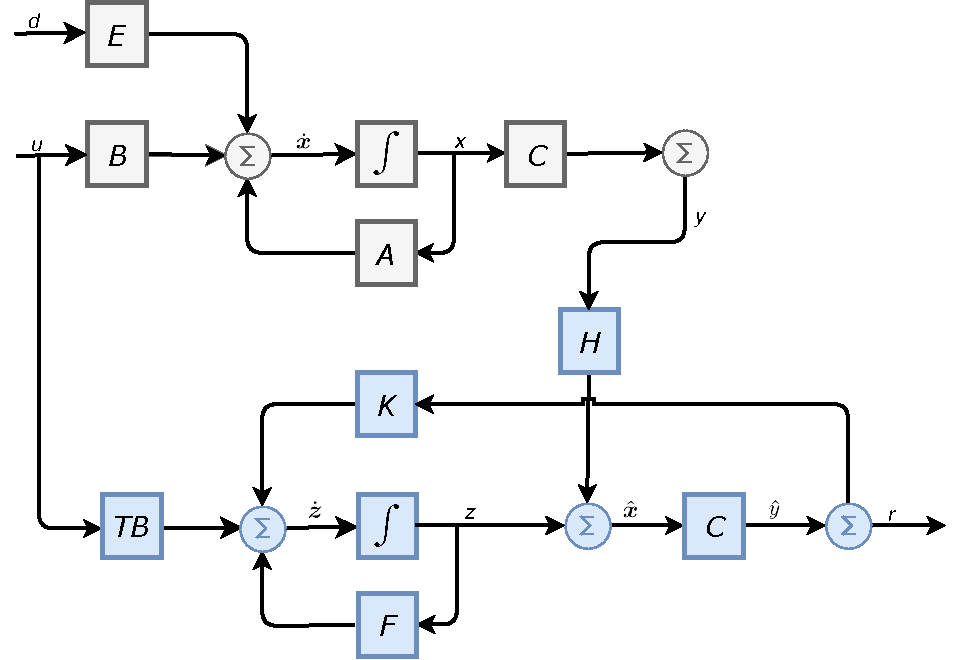
\includegraphics[width=0.8\linewidth]{figures/UIO}
	\caption{Observer based residual generator}
	\label{fig:residualobs}
\end{figure}
Moreover, in the \figref{fig:residualobstest} it can be seen how the state error converge asymptotically to zero from the initial conditions along with a change in the attitude of the satellite after 70 seconds.
\begin{figure}[H]
	\centering
	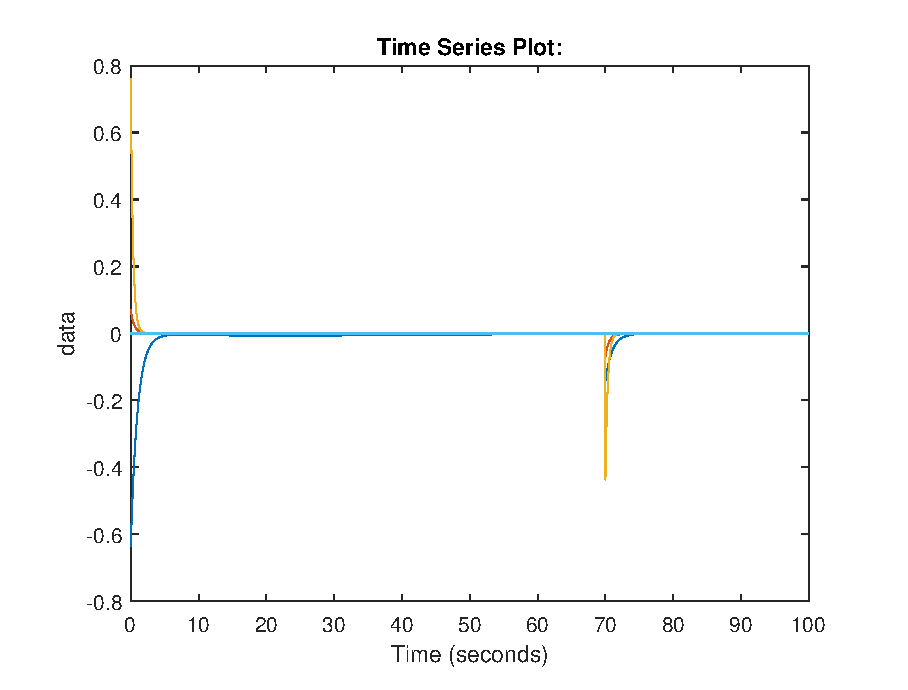
\includegraphics[width=0.7\linewidth]{figures/obstest}
	\caption{Convergence of the state estimation error to zero with the disturbance been decoupled}
	\label{fig:residualobstest}
\end{figure}
 Fault isolation is possible assuming that all the sensors are fault free. A descriptor model of the overall system with actuator fault can be written as \eqref{stateObs} by adding the actuator fault indicator in the equation as 
\begin{equation}
\dot{\vec{x}} = \underline A\vec{x}+\underline B \vec{u}+\underline E\vec{d} + \underline B\vec{f_{act}}
\label{stateObs34}
\end{equation}
where $\vec{f_{act}}$ represents the actuator faults. After the detection, faults can be isolated by deleting the $i_{th}$ column of the matrix B namely $\vec{b_{i}}$ and incorporating this along with the disturbance distribution matrix as
\begin{equation*}
E^{i} = [ E  \vec{b_{i}}]
\label{errordynamics14}
\end{equation*}
and furthermore, the $i_{th}$ component of the input vector $u_{i}$ is incorporated to the disturbance vector as 
\begin{flalign*}
\begin{bmatrix}
\vec{d} \\ u_{i}+f^{i}_{act}
\end{bmatrix}
\end{flalign*} 
leading to a bank of observers with each residual actuated by 2 inputs(without $i_{th}$) and all outputs. The detection of the fault is made by applying a threshold as  $\{\lVert r^{i}\rVert < Thr^{i} \}$ else if $\{\lVert r^{k}\rVert \geq Thr^{k} \}$ with $k = 1,...i-1,..i+1,5..r$.
%\subsection{CUSUM algorithm and change detection} 
%The evaluation of the residual which determines if the %actuator is faulty or fault free is based on the %cumulative sum (CUSUM), a sequential hypothesis %testing technique to detect changes on the noisy %signal. By changes are accounted changes on the mean %of the original signal. 



% \begin{figure}[H]
%	\centering
% 	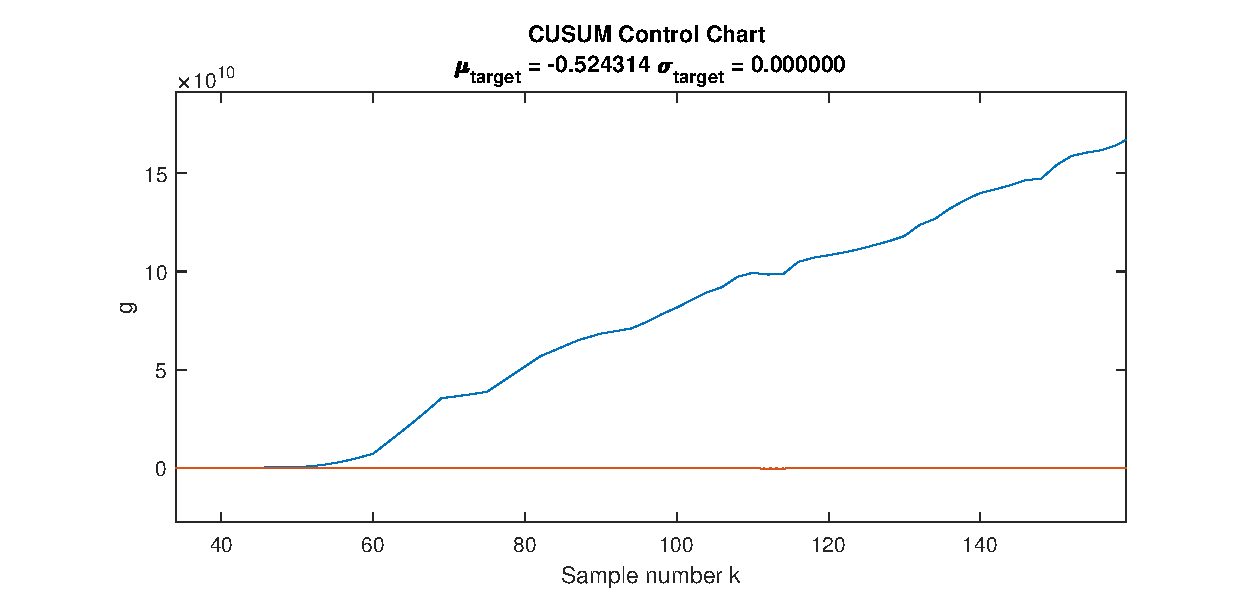
\includegraphics[width=0.7\linewidth]{figures/cusum1}
% 	\caption{CUSUM output with fault on the z axis magnetorquer at 40s }
%	\label{fig:cusum1}
%\end{figure}  

